\begin{figure*}
    \centering
    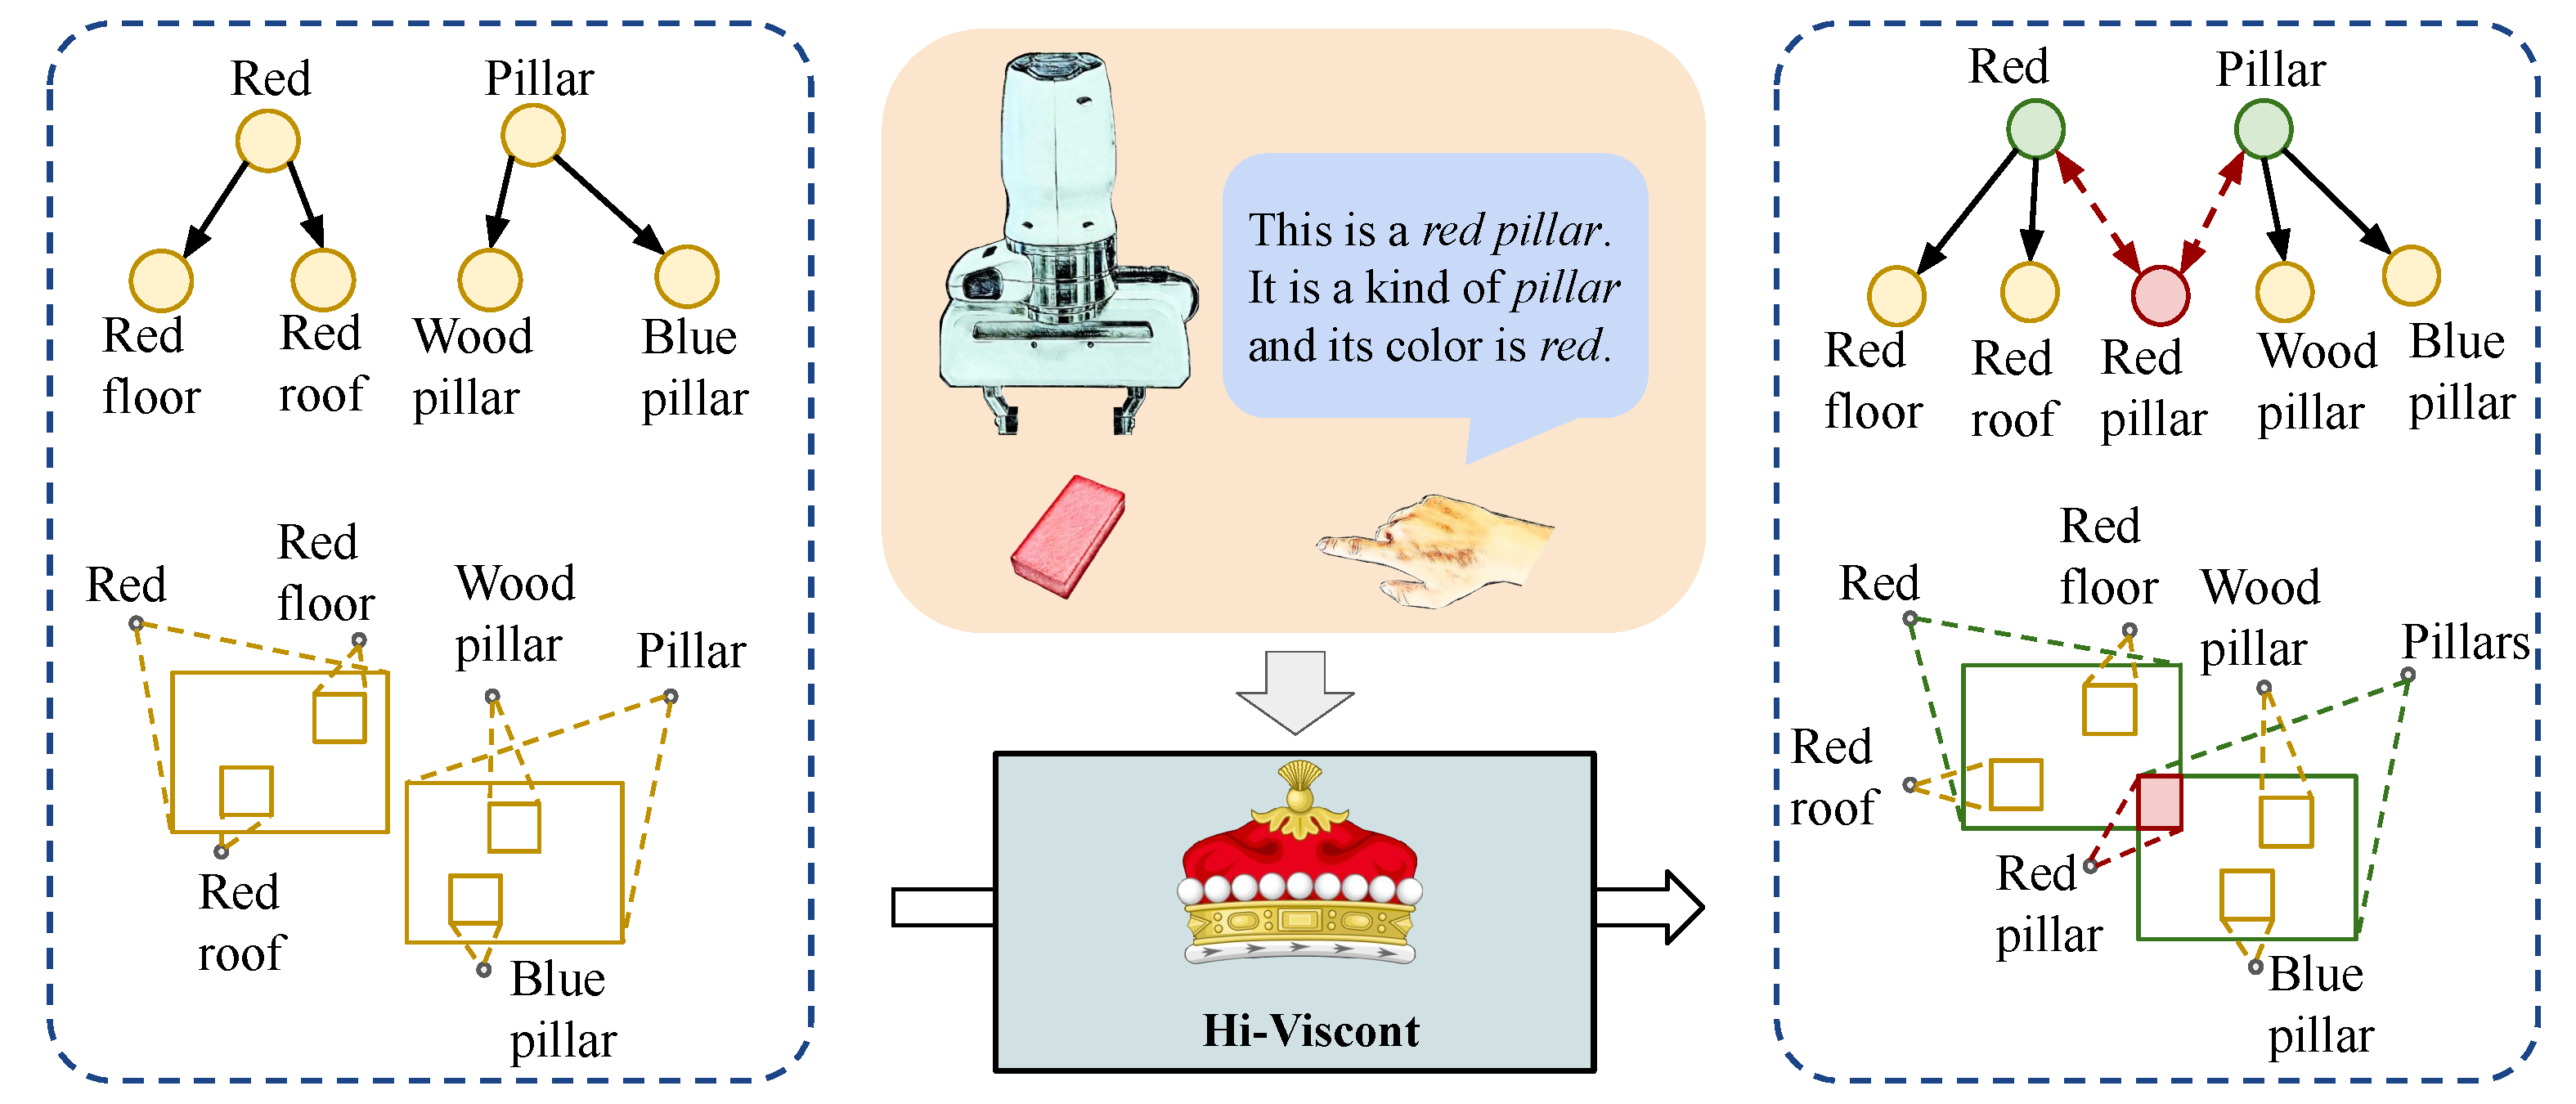
\includegraphics[width=0.75\textwidth]{figures/figure2.pdf}
    \caption{We demonstrate the updates to the box embedding space and the parent concepts when a novel concept is taught to our robot using Hi-Viscont. Existing approaches only edit the leaf nodes as those represent novel concepts.}
    \label{fig:concept_net_model}
    % \vspace{-5mm}
\end{figure*}

% introduce FALCON
% With more details, this should take about 3/4 of a column
We first present the baseline FALCON model and then introduce our Hi-Viscont model. Our model is based on concept learners as they learn concepts few shot, and can reason over the attributes of chosen (and their parent) concept classes. FALCON is a State-of-the-art (SOTA) concept learner which learns novel concepts one-shot. 
% Details for why FALCON
% The ability of learning concepts on the fly is necessary for robots to perform tasks because robots will run into unknown objects or concepts when they are performing the task, and such ability can quickly adapt robots to unseen tasks.
% Therefore, we hope to adopt one-shot learning framework to the robotic domain.


\subsection{FALCON}
% The task that FALCON solves
%   One-shot visual concept learning
%   Answer visual reasoning questions
\citet{mei2022falcon} developed FALCON, a meta-learning framework for one-shot concept learning in visual domains.
FALCON learns a new visual concept with one or a few examples, and uses the learned concept to answer visual reasoning questions on unseen images.
There are three components for the model: a visual feature extractor that extracts the object-centric features for the input image, a graph neural network (GNN) based concept learner, and a neuro-symbolic program executor that executes the input neuro-symbolic program.


% go through a bit the neuro-symbolic programs
Natural language sentences describing objects and their queries are represented as structured neuro-symbolic programs.
FALCON learns novel concepts by interpreting the images presented and the relationships between known concepts and the unknown concept being learned using a neuro-symbolic program. 
After learning, the model performs reasoning over questions, executed as neuro-symbolic programs to answer questions about images. 
% By executing these neuro-symbolic programs, FALCON learns novel concept by interpreting the image and the relations with other known concepts, and performs reasoning on visual reasoning questions.
% FALCON's visual feature extractor


A pre-trained ResNet-34 is used as visual feature extractor for the model.
% The input to the visual feature extractor is the mask for each object of the image and the original image.
The visual feature extractor computes a feature for each object in a scene separately, which can be used for downstream visual reasoning.
% Box embedding
FALCON uses a box embedding\citep{vilnis2018probabilistic} to represent concepts and their object visual features.


%In the box embedding space, a concept is represented as a high dimension box. The embedding of a concept is a tuple of two vectors: $e_c = (\text{Cen}(e_c), \text{Off}(e_c))$, denoting the center and the offset of the box embedding.
% GNN 
% \asnote{Is the transition correct}
Finally, the concept learning module is composed of two separate Graph Neural Networks(GNNs), the Relation GNN and the Example GNN.
To compute a representation for a novel concept $c$, FALCON starts with an embedding that is randomly sampled from a prior Dirichlet distribution.
% The example GNN is used to compute a message from the visual feature to the embedding.
Then, the model updates the representation of $c$ by computing messages from parent nodes based on their factor weights or relationship and also computing a message from the visual feature (represented as a node within the Example GNN) for the concept being learned.  
This representation for the novel concept $c$ will then be used for downstream VQA tasks. 
% \citealt{mei2022falcon} trained the concept learning module by using the computed representation of the novel concept $c$ for visual question answering task.
% a message from the related parent concepts to the novel concept based on their relationships using the relational GNN.
% FALCON further updates the representation of $c$ by computing the message from the visual feature of the object that serves as the example of the novel concept to the embedding computed by the relational GNN. The resulted representations are the candidates for the representation of the novel concept $c$.
% FALCON then uses the candidate representation that has the highest data likelihood as the representation of the novel concept $c$, denoted $e_c = e_c^k; k = argmax_i P(e_c^i\mid o^{(c)})$, where $o^{(c)}$ is the visual representation extracted from the train image, $e_c^i$ is the candidate embedding for concept $c$, and $e_c$ is the final representation for concept $c$.
% \citealt{mei2022falcon} trained the concept learning module by using the computed representation of the novel concept $c$ for visual question answering task.

%The concept learning module takes the relations between the novel concept and other known concepts, and the visual features of the object that serves as the instance of the novel concept as inputs. 
%Each relation with a known concept $c'$ is a 3-tuple $(c, c', rel)$, where $rel$ denotes the relationship of $c$ with $c'$. We denote the collection of these relations as $R_c$.
%Because the representation for the objects in the example image is also in the same embedding space, FALCON treats them as another related concept to the novel concept $c$ with a special relationship $r_o$. We denote the representation of these objects as $o_c$

%These priors are treated as the initial embedding for the novel concept $c$.
%$GNN_1$, also known as the relational GNN, updates the embedding for concept $c$ by computing a message from the relations $R_c$ to the initial embeddings $e_0^i$. We denote this as $GNN_1(R_c, e_c^{0,i})=e_c^{1,i}$. 
%$GNN_2$, the example GNN, treats the features of the example object of the novel concept $c$ as a related concept to $c$, with a unique relationship. 
%The example GNN then updates the embedding for $c$ by computing the message from the features of the example messages to $e_c^{1, i}$, this process is denoted as $GNN_2()$
 

% Why FALCON is insufficient?
There are two major issues to directly use FALCON for interactive task learning on the robot. Firstly, the model lacks scene information to solve tasks. We address this in our work. Secondly, the model assumes concepts are learned perfectly and do not need to be updated as it learns more concepts.
% Such assumption may not be true under the real world scenario, and the flaw of such design gets more obvious when we have less or no prior knowledge about the concepts.
For example, when we teach the model the concept of ``container'' with an image of a ``cup,'' FALCON cannot update the features of the ``container'' concept when the concept of ``bowl'' is taught as a child to the ``container'' concepts. This allows FALCON to learn that all ``containers'' have handles which is untrue.
\begin{figure*}[h]
    \centering
    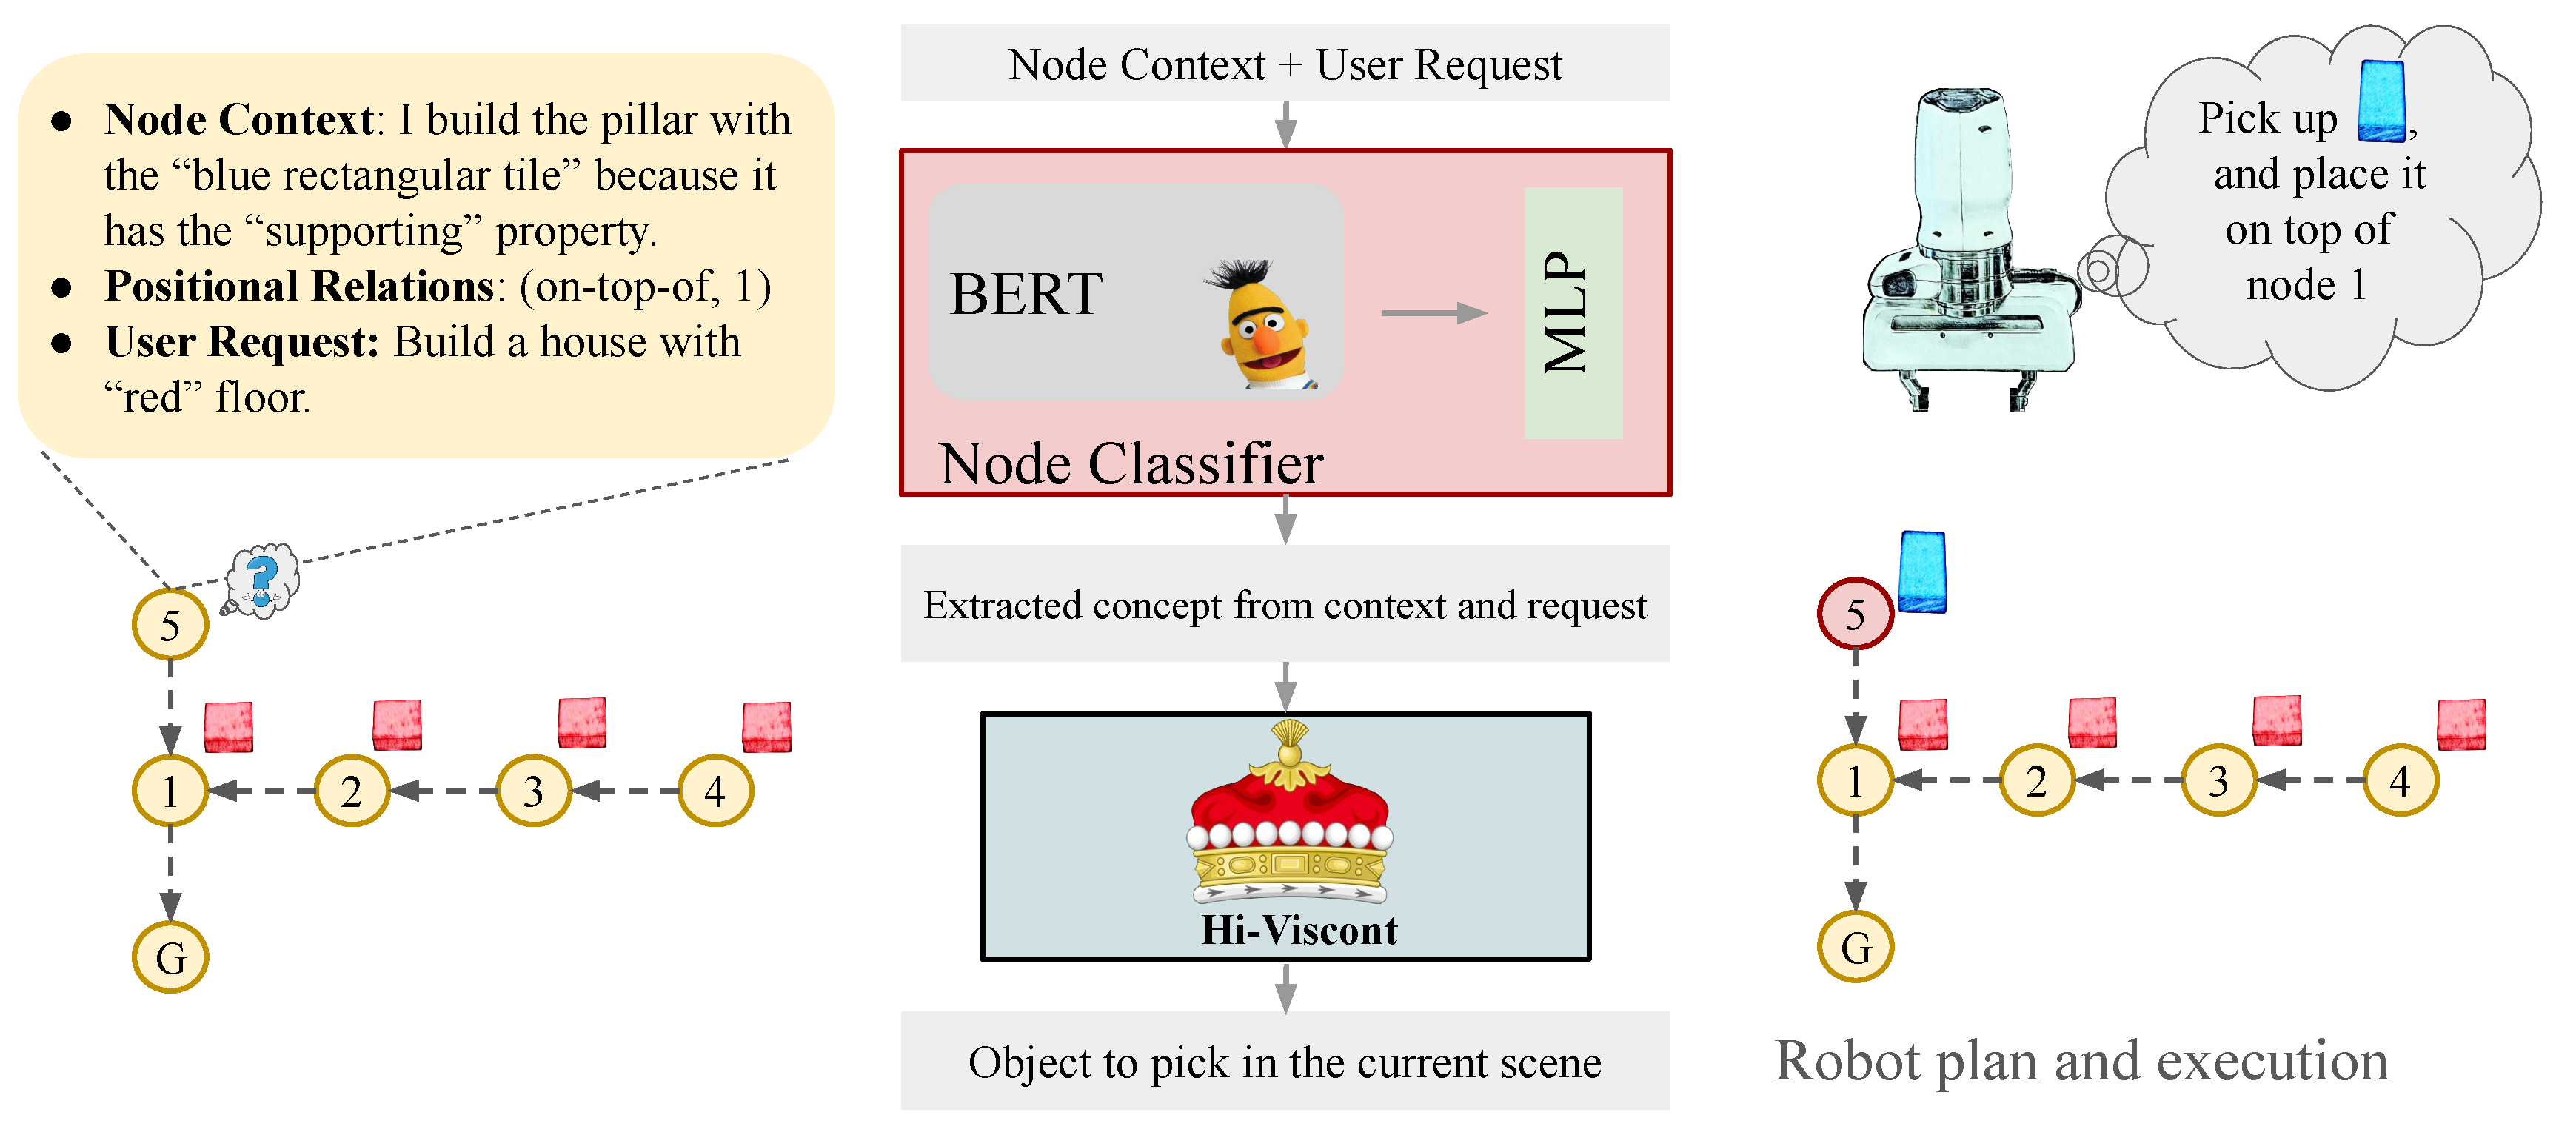
\includegraphics[width=0.75\textwidth]{figures/pipeline_fig.pdf}
    \caption{Our pipeline decides objects for each node in the scene graph one at a time. The node's context and the request phrase are fed into a node classifier, which is composed of a BERT encoder and an multilayer perceptron, to decide the concepts applicable for the current node. Hi-Viscont then decides the object to pick in the current scene based on the extracted concepts. In this example, the object chosen for Node 5 is "blue rectangular tile" as it existed in the original demonstration and was not changed given the novel task's linguistic request. Notice that the new structure has red floor tiles which were never demonstrated to the robot.}
    \label{fig:node_classifier}
\end{figure*}

\subsection{Hi-Viscont}
We present our concept net model, Hi-Viscont (HIerarchical VISual CONcept learner for Task), which actively updates the related known concepts when we introduce the novel concept to improve upon FALCON's generalization capabilities.
% introduce which part we adopted from FALCON
We adopted several modules from the framework of FALCON, including the visual feature extractor, the neuro-symbolic program executor, the box embedding space, and the novel concept learner.
% That is to say, our concept net model learns the representation of the novel concept in the exact same way as FALCON.
% introduce the new gnn
% \asnote{Is this transition fine, can we use In addition to for example, also i think the sentence is gramatically wrong} 
Moreover, we introduce an additional GNN module, Ancestor Relational GNN (ARGNN), that updates the related known concepts as a novel concept is introduced. 
ARGNN predicts a new embedding for the related known ancestor concepts to the novel concept. To do this update we compute a message from the visual feature of novel concept's instance to the embedding of the related nodes using the relations between the parent concepts and the novel concept.
% \wgnote{Describe GNN 3}


When a novel concept $c$ is inserted to Hi-Viscont, the extracted visual feature $o_c$ of concept $c$ and its relations with known concepts $R_c$ are fed to Hi-Viscont as input. 
Each relation $rel=(c',c, r)$, where $c'$ denotes the related concept, and $r$ describes its relationship with $c$.
We compute an embedding $e_c$ for novel concept $c$ using the same method as FALCON.
Using the additional ARGNN, we predict a new embedding for each related concept $c'$ by computing a message from the visual feature $o_c$ to the current embedding of the related concept $e_{c'}^0$ using the same relationship $rel$.
The formula for this update is denoted as follows: $$e_{c'}^1 = \textrm{ARGNN}(o_c, rel, e_{c'}^0)$$
The resulted embedding $e_{c'}^1$ will be used as the representation for concept $c'$ for future task or updates.
% \wgnote{Description ends}



To provide gradient flow to train ARGNN, we extended the concept learning task proposed by FALCON by adding validation questions for each related concept, that is when a new concept is added all concepts in the concept net are tested for accuracy over the novel concept. For example, from our previous discussion the newly inserted ``bowl'' concept's object instance is checked with the ``container'' parent to see if the presented ``bowl'' also tests as a ``container.''   A more detailed description of our training pipeline and  methodology can be found in the appendix.
While FALCON was evaluated solely on the newly inserted concept, we evaluate all concepts (leaf and parent nodes) of our model on unseen images. Such an evaluation ensures consistency between parent and child concepts which is a necessity in continual learning settings. 
This evaluation mechanism allows us to evaluate the quality for the embedding of all concepts in the resulting knowledge graph, which is closer to how these knowledge are used in the real world setting. 





\subsection{Learning Visual Task via Scene Graph}
Figure~\ref{fig:interactive_task_teaching} illustrates how our pipeline learns a visual task from a single in-situ interaction with a human user.
The user's demonstration(Fig.~\ref{fig:interactive_task_teaching}.a) is first converted  into an initial scene graph.
Each node of the initial scene graph corresponds to an object that the user placed, and it contains the bounding box information of the object and the user's linguistic description of the object.
We also store the positional relations with respect to other nodes for each node, which allows for object placements when reconstructing the scene.
% These positional information will be used to compute the placement location of objects when later the robot attempts to reconstruct the scene.
A fixed location on the table is marked with black tape as the origin, which is treated as the zeroth object. All other objects placed by the user will be to the top right of the origin.
% We mark a fixed location with black tape on the table, which serves as the origin and is treated as the zeroth object. All other objects placed by the user will be to the top right of the origin.
% , and the location of the origin is always known to the robot.
% The other nodes will be sorted as an ascending order from bottom to top and from left to right.
%In this work, the positional representations only contain information of directions. 
%When looking for the placement location of an object, we only refer to the relation with its nearest neighbor, and we will place the object in the direction denoted in the relations with a fixed distance. 
%


Based on the initial scene graph and the user's linguistic request for the desired variant of the visual scene, we infer a goal scene graph modelled as a node-wise classification task as shown in Figure~\ref{fig:node_classifier}.
Since the variant of the visual task from the user request shares the same structure as the demonstration, the goal scene graph has the same number of nodes as the initial scene graph.
We take the user's description of the corresponding node of the initial scene graph $t_i$ and the user's request of the variant of the structure $q$ as inputs, and perform a two-step inference: First we decide if the node in the goal graph is different from the one in demonstration; Subsequently if the node is different we decide with classification which object satisfies the node location.


% We perform a binary classification for each node 
To decide whether the concept of a node within the scene has changed given the user's description of the node and the user's current request $q$, we perform a binary classification at each node. The result of this classification decides if we are changing a node's concept or not. 
We use a pretrained BERT\textsubscript{base} model to encode the context request pair, which is then fed into a multi-layer perceptron (MLP) with a Cross-Entropy loss.
% in the format of \\
% $$[CLS] context [SEP] request [SEP]$$
% The embedding of the $[CLS]$ token is treated as the representation for sequence, and is fed into a MLP classifier for the binary classification.
The second step of the inference extracts the related concepts from the context if the node's concept needs to be changed as per the request.
We convert the concept extraction problem into a classification problem by providing concept candidates as a part of the input again with BERT model and an MLP with a Cross-Entropy loss.
The related concepts of each node are fed as input for the concept net model to decide the object to pick, and the positional relations with other nodes are used to compute the placement location.
The robot reconstructs the scene following the order of the nodes.
%For each node, the robot picks the object according to the concept net model.
% Each object is placed at a fixed distance to the direction indicated by the relation with its closest neighbor that is placed.
Pairing the concept net model with scene graph, the robot is able to learn the arrangement of a scene in one single demonstration and perform variants of the scene without demonstration. We allow FALCON access to our Scene Graph classifiers to have a valid baseline to compare against. 



\subsection{Robotics Setup for User Study}
We integrate our visual task learning and concept learning model with a Franka Emika Resarch 3 arm (FR3). 
% Our complete pipeline learns a new object conceptually with the help of its visual features and a description, get a user query to create a new scene, recreate a scene learned from the scene graph learned from the user demonstration with the change mentioned in the query.
This pipeline allows us to show the generalizability with which Hi-Viscont learns visual concepts when compared to Falcon~\cite{mei2022falcon} in learning and solving novel tasks. 
To set this demonstration up we use a Franka Emika Research 3 arm (FR3), two calibrated realsense D435 depth cameras, and a mono-colored table to allow for background subtraction. We use the SAM (Segment Anything Model)~\cite{kirillov2023segment} to separate the foreground and the background and get individual bounding boxes for each of the blocks on the table. 
For pick and place, we initially experimented with Transporter networks~\cite{zeng2021transporter}
% We aimed to create a simple scene-building mechanism that is able to pick objects based on the classification from the place camera frame and rebuild a scene in the scene place in the place camera frame.
but finally used a simpler Visuo-Motor Servoing mechanism for reliability.
We expected users to maintain about an inch of space between each object in the scene to allow the robot to pick objects without collisions and for SAM to segment objects from the background accurately.
In the process of picking and placing, the robot autonomously recovers if an error is made.
%if an error is made the robot recovers autonomously.
Once an object is grasped, we place it into the Task scene based on the position calculated relatively  with respect to the previously placed object nodes or the zeroth origin object. This process is done iteratively until the whole scene graph is completed.


\subsection{Human-Subjects Experiment}
\subsubsection{Study Design}
We conduct a 1 $\times$ 2 within-subject experiment to measure the framework's ability to learn visual task and visual concepts from in-situ interaction.
We extend the FALCON model with our scene graph module and use it as a baseline to compare against because we could not find any equivalent prior work.
Both concept net models are trained with the same split of concepts and the same training data for the same number of steps.
Through this experiment, we aim to demonstrate that our framework achieves better performance than FALCON model because of the continual update for the known knowledge.
Participants for our experiment interact with the robot in three phases.
For each interactive phase, the participants only interact with the robot once, and the interaction is recorded as the input for both systems.
After the interactive phases, the participant observes the two systems construct the scene requested by the participant. Half the participants observe FALCON first and other half observe Hi-Viscont system first to avoid ordering confounds.

% \asnote{Overlap between this and the prior sentence?} The participants observe both systems construct the scene with randomization in the order in which they observe the FALCON or our Hi-Viscont system first.   
% To remove the confounding factor, the participants are into two groups equally, and each group observes the reconstruction of the two systems in different order.
\subsubsection{Human Subjects Experiment Domain}
We evaluate our approach with the human-subjects experiment in a 2-D object rearrangement domain, which is a problem commonly used in language grounding and HRI research~\citep{liu2021structformer, shridhar2021cliport}.
The domain we choose for this study is the House-Construction domain which we introduce in Domains Section. We designed this domain as the users have the ability to create complex types of structures with different object classes.
Building blocks from children's toys were used as objects in this domain as they are varied and easy to grasp by the robot, as grasping is not a focus of our work.

\subsubsection{Metrics}
The objective metrics we collect for the human-subjects experiment are as follows. 
We measure the success rate (SR) of completing the user's request with complete accuracy, and the node level accuracy of each scene graph for both systems.
Both metrics are used to measure each system's ability to actually complete the visual task objectively.
The success rate metric gives us the insight of system's ability of completing the whole task, while the node level accuracy metric provides a more fine-grained result on few-shot object recognition.
% \ngnote{Do subjective tests and cite them here!}
% The subjective metrics we collect for the human-subjects experiment are as follows(the details of hand-crafted surveys, Cronbach's alpha, qualitative results, and quotes from interview questions are in the Appendix).
In the post-study survey for each system, we administer the Perceived Intelligence and Anthropomorphism sub-scales of the Godspeed Questionnaire Series~\cite{Bartneck2009MeasurementIF}, Trust in Automated systems questionnaire~\cite{trust_survey}, System Usability Scale (SUS)\cite{article}.
In addition, we hand-crafted a direct comparison survey for preference between Hi-Viscont and the FALCON model.

\subsubsection{Procedure}
This study was approved by our university's Institutional Review Board (IRB). We recruited all participants through on campus advertisements. 
The study took under $90$ minutes with voluntary participation. The participants were not compensated for their efforts. The procedure of the study is as follows. 
Participants first fill out consent form and then the pre-study survey.
After the pre-study survey, we hand out a general introduction for the experiment of the study.
Then, we guide the participant through the task teaching phase, the concept teaching phase, and the request phase sequentially as described below. 
% We will discuss about the tasks for each of these phases below.
Before each phase, we provide a demonstration video and the instructions of the corresponding phase to the participants. The instruction videos is demonstrating a different task (bridge making) with different objects (foam blocks) than the actual task the participant is teaching. 
The anonymized instruction manual and the link to these videos are provided in the Appendix and the associated webpage~\footnote{\url{https://sites.google.com/view/ivtl}}.

% webpage~\footnote{\url{https://sites.google.com/view/interactivevisualtasklearning/home}}.

\noindent\textbf{Task Teaching Phase - } In the task teaching phase, the participants teach the robot a visual task by demonstrating the scene with its constituent structures one by one. The participants also describe the structures and the objects used to build the structure with natural language. For example, a participant might build a house, with floors, pillars and a roof. While building the roof the participant might say ``This a roof which I build with the curved blue tile because of it's sheltering capability.'' The participants demonstrate each of the structures with their chosen language commands one after another to build a house. We record all descriptions in audio and convert them into text using audio to text tools.  
% which object they choose to build that node, and the reason for choosing such object. 

\noindent\textbf{Concept Teaching Phase - } In this phase, the participants teach a novel concept of their choice to both systems by showing the object to the camera, and describing the concept's properties, such as the color and functional characteristics of the object, in natural language. 
The description to the novel object concept is converted to neuro-symbolic programs, which are given to both models for updates as described in the Methods section. 


\noindent\textbf{Request Phase - } In the request phase, the participants are asked to provide a request in natural language for a novel scene that they did not demonstrate in the task teaching phase. They are instructed to use the object taught in the concept teaching phase in the request. The requested task still needs to be a house which is the same task type as the demonstration, but not a house that the models have seen.


After completing the three phases, the participants watch the two systems construct their requested scene in real time with a robot in a randomized order. As each system finishes the construction, the participants are asked to fill a post-survey for that system. After both systems finish the construction, the participants also fill out a comparative survey.


\subsubsection{Hypotheses}
We have the following hypotheses:


\noindent\textbf{Hypothesis 1 - } Our framework will have a higher success rate in completing the user's request without any errors. We hypothesize that our framework will have a higher success rate than FALCON model because of its update to the related known concepts, which could be used in requests that point to the same object indirectly.


\noindent\textbf{Hypothesis 2 - } Our framework will have a higher node level accuracy. We hypothesize that our framework will achieve a higher accuracy in the node level than the FALCON model as Hi-Viscont can correctly predict the object in a node without direct queries specifying the type of object. FALCON  does not handle these indirect queries well as it does not update parent concepts with knowledge about novel leaf level concepts.


\noindent\textbf{Hypothesis 3 - } We hypothesize that our framework will achieve higher ratings on subjective metrics compared to the baseline because of its higher accuracy and competency in completing the requests. 
